% ----------------------------------------------------------------
% AMS-LaTeX Paper ************************************************
% **** -----------------------------------------------------------
\documentclass[10pt]{amsart}
\usepackage{graphicx, mathabx, amssymb,amsfonts,amsmath,amsthm,newlfont}
\usepackage{epsfig,url}
\usepackage[usenames,dvipsnames]{color}
\usepackage{enumerate}
\usepackage[colorlinks=true,linkcolor=red,citecolor=blue]{hyperref}
\usepackage{color}


%Clever ref
\usepackage[noabbrev,capitalize]{cleveref}


\usepackage[all,2cell]{xy} \UseAllTwocells \SilentMatrices


% ----------------------------------------------------------------
\vfuzz2pt % Don't report over-full v-boxes if over-edge is small
\hfuzz2pt % Don't report over-full h-boxes if over-edge is small
% THEOREMS -------------------------------------------------------
\newtheorem{thm}{Theorem}[section]
\newtheorem{corollary}[thm]{Corollary}
\newtheorem{lemmma}[thm]{Lemma}
\newtheorem{proposition}[thm]{Proposition}
\newtheorem{Questions}[thm]{Questions}
\theoremstyle{definition}
\newtheorem{definition}[thm]{Definition}

\newtheorem{conjectue}{Conjecture} 
\newtheorem{QQ}{Question} 
\newtheorem{prob}{Problem}
\newtheorem{ex}[thm]{Examples}
\newtheorem{example}[thm]{Example}
\newtheorem{policy}{Policy}
\theoremstyle{remark}
\newtheorem{rem}[thm]{Remark}
\newtheorem{caveat}[thm]{Caveat}
\numberwithin{equation}{section}
% MATH -----------------------------------------------------------
\newcommand{\norm}[1]{\left\Vert#1\right\Vert}
\newcommand{\abs}[1]{\left\vert#1\right\vert}
\newcommand{\set}[1]{\left\{#1\right\}}

\newcommand{\To}{\longrightarrow}
\newcommand*{\Longhookrightarrow}{\ensuremath{\lhook\joinrel\relbar\joinrel\rightarrow}}
\newcommand{\Z}{\mathbb Z}
\newcommand{\Q}{\mathbb Q}
\newcommand{\C}{\mathbb C}
\newcommand{\Ok}{\mathcal O}
\newcommand{\ai}{\mathfrak{a}}
\newcommand{\bi}{\mathfrak{b}}
\newcommand{\R}{\mathbb R}
\newcommand{\N}{\mathbb N}
\newcommand{\AM}{A}
\newcommand{\xx}{\mathsf{x}}
\newcommand{\eqv}{\mathrm{ev}}
\font \rus= wncyr10
\newcommand{\sha}{\, \hbox{\rus x} \,}

\newcommand{\Lie}{\mathrm{Lie}}

\newcommand{\GC}{\mathcal{GC}}
\newcommand{\q}{/\!/}

\newcommand{\tr}{\mathrm{tr}}
\newcommand{\id}{\mathrm{id}}

\newcommand{\can}{\mathrm{can}}

\newcommand{\mm}{\mathfrak{m}}

\newcommand{\GL}{\mathrm{GL}}
\newcommand{\LP}{L}
\newcommand{\FL}{F\!L}
\newcommand{\mc}{\mu}


\newcommand{\0}{\color{blue}{\mathsf{0}}}

%Drapeau européen

\usepackage{graphicx,calc}
\newlength\myheight
\newlength\mydepth
\settototalheight\myheight{Xygp}
\settodepth\mydepth{Xygp}
\setlength\fboxsep{0pt}
\newcommand*\inlinegraphics[1]{%
  \settototalheight\myheight{Xygp}%
  \settodepth\mydepth{Xygp}%
  \raisebox{-\mydepth}{\includegraphics[height=\myheight]{#1}}%
}

%Dessins

\usepackage{tikz}
\usepackage{tikz-cd}
\usepackage{pgfplots}
\usepackage{pgfplotstable}
\tikzset{math3d/.style=
    {x= {(-0.353cm,-0.353cm)}, z={(0cm,1cm)},y={(1cm,0cm)}}}
\tikzset{JLL3d/.style=
    {x= {(0.4cm,-0.2cm)}, z={(0cm,1cm)},y={(-1cm,0cm)}}}
\usetikzlibrary{calc}
\usetikzlibrary{shapes,shapes.geometric,fit,positioning,calc,matrix}
\tikzset{
  optree/.style={scale=.5,thick,grow'=up,level distance=10mm,inner sep=1pt},
  comp/.style={draw=none,circle,fill,line width=0,inner sep=0pt},
  dot/.style={draw,circle,fill,inner sep=0pt,minimum width=3pt},
  circ/.style={draw,circle,inner sep=1pt,minimum width=4mm},
  emptycirc/.style={draw,circle,inner sep=1pt,minimum width=2mm},
  root/.style={level distance=10mm,inner sep=1pt},
  leaf/.style={draw=none,circle,fill,line width=0,inner sep=0pt},
  nodot/.style={draw,circle,inner sep=1pt},
}

\pgfplotsset{compat=1.12}

% ----------------------------------------------------------------

\def\abovespace{\vspace{12pt}}
\def\belowspace{\vspace{8pt}}



\addtolength{\hoffset}{-0.0in} \addtolength{\textwidth}{0in}
\addtolength{\voffset}{-0.0in} \addtolength{\textheight}{0.0in}


% -----------------------------------------------------------------

\title{Categorified operads, polytopes and Koszulity}

\author{Pierre-Louis Curien}
\address{IRIF, Universit\'e Paris Diderot and $\pi r^2$ team, Inria, France.}
\email{curien@irif.fr}

\author{Guillaume Laplante-Anfossi}
\address{Universit\'e Sorbonne Paris Nord, Laboratoire Analyse, G\'eom\'etrie et Applications, CNRS, UMR 7539, F-93430 Villetaneuse, France.}
\email{laplante-anfossi@math.univ-paris13.fr}



\date{\today}

\subjclass[2010]{Primary [...]; Secondary 18M70} 

\keywords{Polytopes [...]}

\dedicatory{"We shall construct $KP_n$, as a CW-complex, in Section 2 and show that it is an $(n-1)$-ball. This gives an instant one-step proof of MacLane's theorem in full generality."  \\ --  Mikhail M. Kapranov}

\thanks{The second author was supported by the European Union's Horizon 2020 research and innovation program under the Marie Sklodowska-Curie grant agreement No 754362 \inlinegraphics{EU.png}, by the Natural Sciences and Engineering Research Council of Canada (NSERC) and by the ANR-20-CE40-0016 Higher Algebra, Geometry and Topology.}

\begin{document}


\begin{abstract}
The purpose of this note is to provide a new 
\end{abstract}


\maketitle

\section{Introduction}

\begin{enumerate}
    \item We introduce a new notion of categorified non-symmetric (ns) operad. We prove that this notion is equivalent the one of weak Cat-operad, introduced by K. Do{\v s}en and Z. Petri{\'c} in \cite{DP15}. 

    \item We prove a generalization of MacLane's coherence theorem for categorified ns operads. We use explicitly the fact that the diagrams associated to a categorified ns operad are 1-skeletons of a family of polytopes, the operahedra. We thus make Kapranov's claim into a theorem. 
    
    \item We use the rewriting method to prove that the operad encoding ns operads is Koszul, and observe that this provides an alternative proof of the preceding coherence theorem. 

\end{enumerate}

\section{Categorified non-symmetric operads}


\begin{definition}[Categorified non-symmetric operad] A \emph{categorified non-symmetric operad} $\mathcal{P}$ is a collection $\left\{  \mathcal{P}(n)  \right\}_{n\in \mathbb{N}}$ of small categories equipped with bifunctors  
$$ \begin{array}{clll}
\circ_i&\colon& \mathcal{P}(n) \times
                  \mathcal{P}(k)
                  \longrightarrow \mathcal{P}(n+k-1) \ ,
                  & \text{for}\ 1 \leq i \leq n \ ,
\end{array}  $$
an object $\mathrm{id} \in \mathcal{P}(1)$ called \emph{unit}, and for each $\kappa \in \mathcal{P}(m)$,  $\mu \in \mathcal{P}(n)$, $\nu \in \mathcal{P}(k)$ natural isomorphisms 
$$ \begin{array}{clll}
    \beta_{\kappa,\mu,\nu}&\colon& 
    (\kappa \circ_i \mu) \circ_{j+i-1} \nu  \overset{\cong}{\longrightarrow} \kappa \circ_i (\mu \circ_j \nu) \ , &  \\
    \theta_{\kappa,\nu,\mu}&\colon& 
    (\kappa \circ_i \nu) \circ_{j+k-1} \mu 
    \overset{\cong}{\longrightarrow} (\kappa \circ_j \mu) \circ_i \nu \ , & \text{when}\ i < j \ , \\
    \lambda_\nu &\colon& 
    \mathrm{id} \circ_1 \nu \overset{\cong}{\longrightarrow} \nu \ , & \\
    \rho_\mu &\colon& 
    \mu \circ_i \mathrm{id} \overset{\cong}{\longrightarrow} \mu \ , & 
\end{array}  $$
such that the following diagrams commute: the triangle \\
\begin{center}
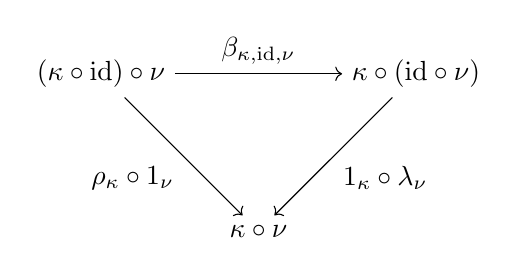
\begin{tikzpicture}[scale=2]
    \node (P1) at (-1,1) {$(\kappa \circ \mathrm{id})\circ \nu$};
    \node (P2) at (1,1) {$\kappa \circ (\mathrm{id}\circ \nu)$};
    \node (P3) at (0,0) {$\kappa \circ \nu$};
    \draw[->] (P1)--(P2) node[midway,above] {$\beta_{\kappa,\mathrm{id},\nu}$};
    \draw[->] (P1)--(P3) node[midway,below left] {$\rho_\kappa\circ 1_\nu$};
    \draw[->] (P2)--(P3) node[midway,below right] {$1_\kappa \circ \lambda_\nu$};
\end{tikzpicture} \quad \quad 
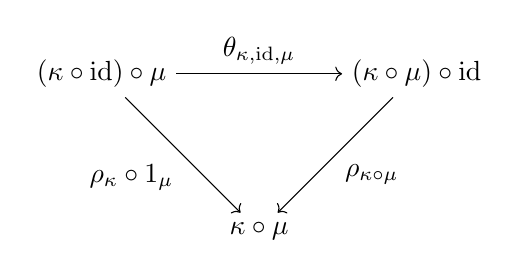
\begin{tikzpicture}[scale=2]
    \node (P1) at (-1,1) {$(\kappa \circ \mathrm{id})\circ \mu$};
    \node (P2) at (1,1) {$(\kappa\circ \mu)\circ\mathrm{id}$};
    \node (P3) at (0,0) {$\kappa \circ \mu$};
    \draw[->] (P1)--(P2) node[midway,above] {$\theta_{\kappa,\mathrm{id},\mu}$};
    \draw[->] (P1)--(P3) node[midway,below left] {$\rho_\kappa\circ 1_\mu$};
    \draw[->] (P2)--(P3) node[midway,below right] {$\rho_{\kappa\circ\mu}$};
\end{tikzpicture} \quad \ ,
\end{center}
pentagonal \\
\resizebox{\linewidth}{!}{
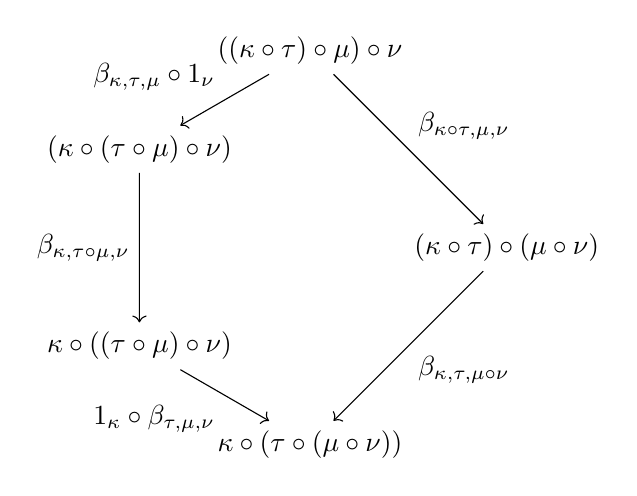
\begin{tikzpicture}[scale=2.5]
    \node (P1) at (0,1) {$((\kappa\circ\tau)\circ\mu)\circ\nu$};
    \node (P2) at (-0.866,0.5) {$(\kappa\circ(\tau\circ\mu)\circ\nu)$};
    \node (P3) at (-0.866,-0.5) {$\kappa\circ((\tau\circ\mu)\circ\nu)$};
    \node (P4) at (0,-1) {$\kappa\circ(\tau\circ(\mu\circ\nu))$};
    \node (P5) at (1,0) {$(\kappa\circ\tau)\circ(\mu\circ\nu)$} ;
    \draw[->] (P1)--(P2) node[midway,above left] {$\beta_{\kappa,\tau,\mu}\circ 1_\nu$};
    \draw[->] (P2)--(P3) node[midway,left] {$\beta_{\kappa,\tau\circ\mu,\nu}$};
    \draw[->] (P3)--(P4) node[midway,below left] {$1_\kappa \circ \beta_{\tau,\mu,\nu}$};
    \draw[->] (P1)--(P5) node[midway,above right] {$\beta_{\kappa\circ\tau,\mu,\nu}$};
    \draw[->] (P5)--(P4) node[midway,below right] {$\beta_{\kappa,\tau,\mu\circ\nu}$};
\end{tikzpicture} \quad 
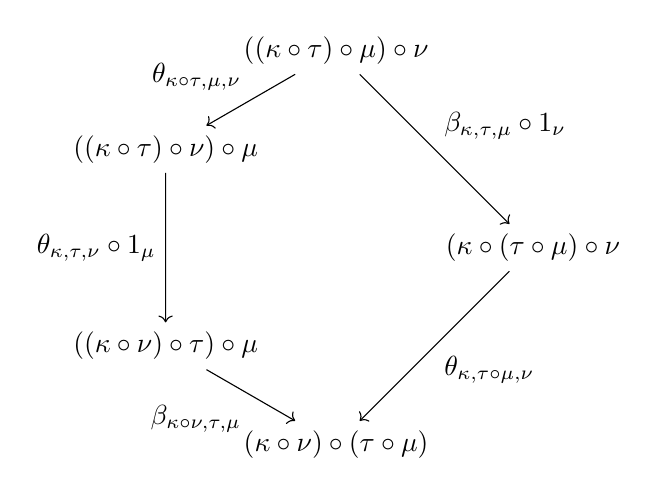
\begin{tikzpicture}[scale=2.5]
    \node (P1) at (0,1) {$((\kappa\circ\tau)\circ\mu)\circ\nu$};
    \node (P2) at (-0.866,0.5) {$((\kappa\circ\tau)\circ\nu)\circ\mu$};
    \node (P3) at (-0.866,-0.5) {$((\kappa\circ\nu)\circ\tau)\circ\mu$};
    \node (P4) at (0,-1) {$(\kappa\circ\nu)\circ(\tau\circ\mu)$};
    \node (P5) at (1,0) {$(\kappa\circ(\tau\circ\mu)\circ\nu$} ;
    \draw[->] (P1)--(P2) node[midway,above left] {$\theta_{\kappa\circ\tau,\mu,\nu}$};
    \draw[->] (P2)--(P3) node[midway,left] {$\theta_{\kappa,\tau,\nu}\circ 1_\mu$};
    \draw[->] (P3)--(P4) node[midway,below left] {$\beta_{\kappa\circ\nu,\tau,\mu}$};
    \draw[->] (P1)--(P5) node[midway,above right] {$\beta_{\kappa,\tau,\mu}\circ 1_\nu$};
    \draw[->] (P5)--(P4) node[midway,below right] {$\theta_{\kappa,\tau\circ\mu,\nu}$};
\end{tikzpicture} \quad 
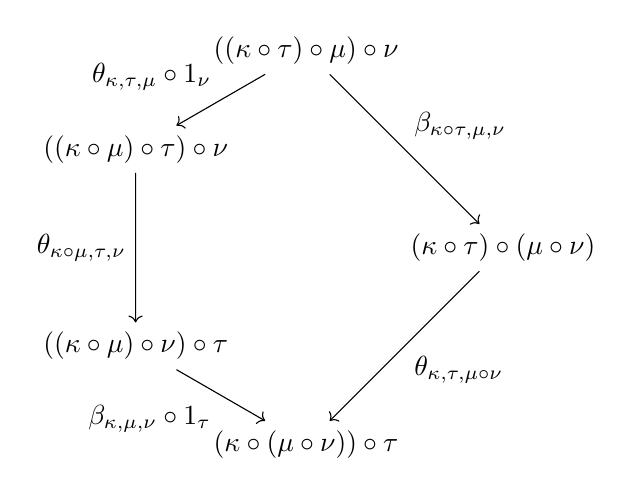
\begin{tikzpicture}[scale=2.5]
    \node (P1) at (0,1) {$((\kappa\circ\tau)\circ\mu)\circ\nu$};
    \node (P2) at (-0.866,0.5) {$((\kappa\circ\mu)\circ\tau)\circ\nu$};
    \node (P3) at (-0.866,-0.5) {$((\kappa\circ\mu)\circ\nu)\circ\tau$};
    \node (P4) at (0,-1) {$(\kappa\circ(\mu\circ\nu))\circ\tau$};
    \node (P5) at (1,0) {$(\kappa\circ\tau)\circ(\mu\circ\nu)$} ;
    \draw[->] (P1)--(P2) node[midway,above left] {$\theta_{\kappa,\tau,\mu}\circ 1_\nu$};
    \draw[->] (P2)--(P3) node[midway,left] {$\theta_{\kappa\circ\mu,\tau,\nu}$};
    \draw[->] (P3)--(P4) node[midway,below left] {$\beta_{\kappa,\mu,\nu}\circ 1_\tau$};
    \draw[->] (P1)--(P5) node[midway,above right] {$\beta_{\kappa\circ\tau,\mu,\nu}$};
    \draw[->] (P5)--(P4) node[midway,below right] {$\theta_{\kappa,\tau,\mu\circ\nu}$};
\end{tikzpicture} } \\
and hexagonal identities \\
\begin{center}
\resizebox{0.8\linewidth}{!}{
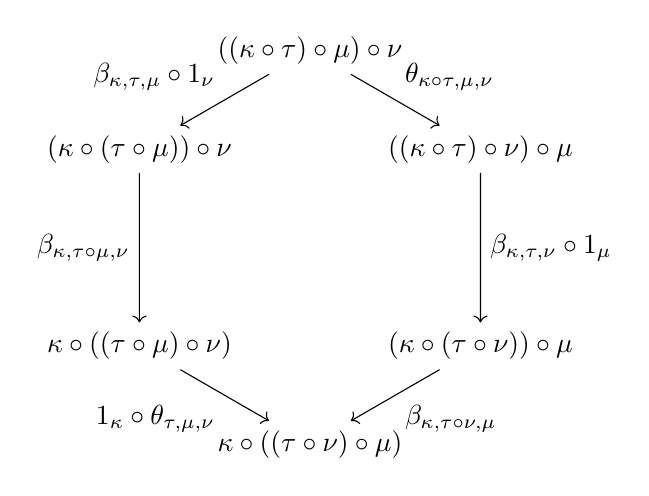
\begin{tikzpicture}[scale=2.5]
    \node (P1) at (0,1) {$((\kappa\circ\tau)\circ\mu)\circ\nu$};
    \node (P2) at (-0.866,0.5) {$(\kappa\circ(\tau\circ\mu))\circ\nu$};
    \node (P3) at (-0.866,-0.5) {$\kappa\circ((\tau\circ\mu)\circ\nu)$};
    \node (P4) at (0,-1) {$\kappa\circ((\tau\circ\nu)\circ\mu)$};
    \node (P5) at (0.866,0.5) {$((\kappa\circ\tau)\circ\nu)\circ\mu$} ;
    \node (P6) at (0.866,-0.5) {$(\kappa\circ(\tau\circ\nu))\circ\mu$};
    \draw[->] (P1)--(P2) node[midway,above left] {$\beta_{\kappa,\tau,\mu}\circ 1_\nu$};
    \draw[->] (P2)--(P3) node[midway,left] {$\beta_{\kappa,\tau\circ\mu,\nu}$};
    \draw[->] (P3)--(P4) node[midway,below left] {$1_\kappa \circ \theta_{\tau,\mu,\nu}$};
    \draw[->] (P1)--(P5) node[midway,above right] {$\theta_{\kappa\circ\tau,\mu,\nu}$};
    \draw[->] (P5)--(P6) node[midway,right] {$\beta_{\kappa,\tau,\nu}\circ 1_\mu$};
    \draw[->] (P6)--(P4) node[midway,below right] {$\beta_{\kappa,\tau\circ\nu,\mu}$};
\end{tikzpicture} \quad \quad
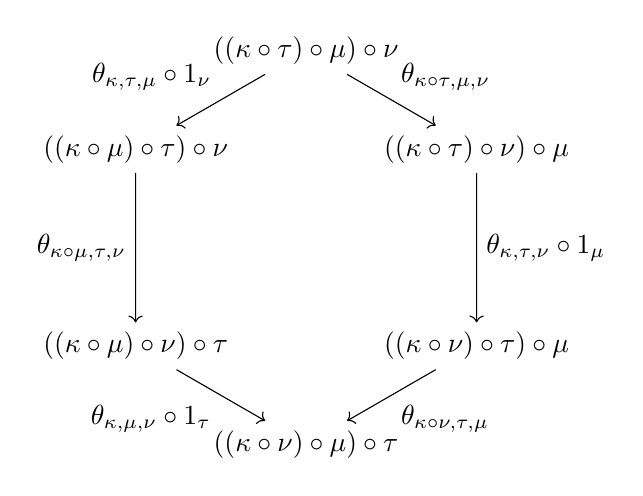
\begin{tikzpicture}[scale=2.5]
    \node (P1) at (0,1) {$((\kappa\circ\tau)\circ\mu)\circ\nu$};
    \node (P2) at (-0.866,0.5) {$((\kappa\circ\mu)\circ\tau)\circ\nu$};
    \node (P3) at (-0.866,-0.5) {$((\kappa\circ\mu)\circ\nu)\circ\tau$};
    \node (P4) at (0,-1) {$((\kappa\circ\nu)\circ\mu)\circ\tau$};
    \node (P5) at (0.866,0.5) {$((\kappa\circ\tau)\circ\nu)\circ\mu$} ;
    \node (P6) at (0.866,-0.5) {$((\kappa\circ\nu)\circ\tau)\circ\mu$};
    \draw[->] (P1)--(P2) node[midway,above left] {$\theta_{\kappa,\tau,\mu}\circ 1_\nu$};
    \draw[->] (P2)--(P3) node[midway,left] {$\theta_{\kappa\circ\mu,\tau,\nu}$};
    \draw[->] (P3)--(P4) node[midway,below left] {$\theta_{\kappa,\mu,\nu}\circ 1_\tau$};
    \draw[->] (P1)--(P5) node[midway,above right] {$\theta_{\kappa\circ\tau,\mu,\nu}$};
    \draw[->] (P5)--(P6) node[midway,right] {$\theta_{\kappa,\tau,\nu}\circ 1_\mu$};
    \draw[->] (P6)--(P4) node[midway,below right] {$\theta_{\kappa\circ\nu,\tau,\mu}$};
\end{tikzpicture}  } \quad \ .
\end{center}
\end{definition}

A categorified ns operad concentrated in arity 1 is a monoidal category.

\begin{definition}[Weak Cat-operad {\cite{DP15}}]
\end{definition}

\begin{thm} \label{thm:equivalenceDPGLA}
    The data of a categorified ns operad and the data of a weak Cat-operad are equivalent.  
\end{thm}

\begin{proof}
    TBC
\end{proof}

\section{Coherence for categorified operads}

Recall from [REF] the definition of the $\mathbb{N}$-colored operad $\mathcal{O}$ encoding ns operads. Its minimal resolution is given by the cellular chains on the operahedra [DEF]. 



\begin{thm}[Coherence theorem] \label{thm:coherence}
    Every diagram with vertices iterates of the $\circ_i$ and edges expansions of instances of $\beta, \theta, \lambda$ and $\rho$ arrows is commutative. 
\end{thm}

\begin{proof} TBC
\end{proof}

Restricted to categorified ns operad concentrated in arity 1, i.e. to monoidal categories, we recover MacLane's original coherence tbeorem [REF].

There is an analogous statement for weak Cat-operads \cite[Proposition 14.2]{DP15}. In the same fashion as for \cref{thm:equivalenceDPGLA}, one can prove that the two statements are equivalent. 

\section{Koszulity}

Let us take a detour by the Koszul duality theory for operads. One of the standard method for proving that an operad is Koszul is the "rewriting method" \cite[Section 8.3]{LodayVallette12}. The generalization to the colored case was done recently by V. Kharitonov and A. Khoroshkin \cite[Theorem 3.12]{KhariKhoro20}.

\begin{thm}[Rewriting method for colored operads {\cite[Theorem 8.3.1]{LodayVallette12}}] \label{thm:rewriting} Let $\mathcal{O}(E,R)$ be a quadratic colored operad. If its generating space $E$ admits a $\mathbb{K}$-linear ordered basis, for which there exists a suitable order on shuffle trees, such that every critical monomial is confluent then the colored operad $\mathcal{O}$ is Koszul. 
\end{thm}

In this case, the operad $\mathcal{O}$ admits an induced shuffle tree basis sharing nice properties, called a PBW basis, see \cite[Section 8.5.3]{LodayVallette12}. Parler Grobner Basis

\begin{thm} \label{thm:Koszulrewriting} The colored operad $\mathcal{O}$ is a Koszul colored operad. 
\end{thm}
\begin{proof} The partial order on complete nested trees defined in X induces, via the proof of X, a suitable order on shuffle trees, see X. The 1-skeleton of operahedra appears as the application of the rewriting rules given by the sequential and parallel axioms. We consider the family of trees $F=\{\tau \in \mathrm{OT}=\ | \ |V(\tau)|=4\}$ and the oriented operahedra $\{(P_\tau,\vec v)\}_{\tau \in F}$ for any vector $\vec v=(v_1,v_2,v_3)$ such that $v_1>v_2>v_3$. Every critical monomial corresponds to the complete nested trees associated to $\{bot(P_\tau,\vec v)\}_{\tau \in F}$, and X implies that every critical monomial is confluent. We conclude by \cref{thm:rewriting}. 
The complete nested trees associated to $\{top(P_\tau, \vec v)\}_{\tau \in F}$ form the PBW basis of $\mathcal{O}_{ns}$.
\end{proof}

The proof of \cref{thm:rewriting} relies on the Diamond Lemma \cite[Theorem 8.5.5]{LodayVallette12}. Instead, we can use the full power of X.

\begin{proof}[Second proof] Every rewriting diagram associated to a monomial is part of the 1-skeleton of some operahedron of dimension $n\geq 0$. By X, this 1-skeleton is oriented and forms the boundary of a topological $n$-ball. Thus, it has a unique maximal element. 
\end{proof}

Restricting to linear trees, we have that the operad $\mathrm{Ass}$ is Koszul. Restricting to the 2-leveled trees as in X, we obtain that the permutad $\mathrm{permAs}^h$ is Koszul, in the sense of M. Markl \cite[Definition 21]{Markl19}.

\medskip

\cref{thm:Koszulrewriting} gives an alternative proof of \cref{thm:coherence}. 

\begin{proof}[Second proof of {\cref{thm:coherence}}] Let $\mathcal{O}$ be a non-unital categorified ns operad. The pentagonal and hexagonal diagrams commute, and they correspond precisely to the 1-skeleton of the 2-dimensional oriented operahedra $\{(P_\tau,\vec v)\}_{\tau \in F}$. Using the Diamond Lemma as in the proof of \cref{thm:rewriting}, we have that every diagram made up of $\theta$ and $\beta$ arrows commute. 
\end{proof}

Here again, resorting to the Diamond Lemma is not necessary.

\begin{proof}[Third proof of {\cref{thm:coherence}}] Any diagram $D$ made up of $\theta$ and $\beta$ arrows lives on the 1-skeleton of an operahedron of some dimension $n\geq 0$. As this operahedron is topologically a $n$-dimensional ball, the diagram $D$ is obtained by gluing together 1-skeletons of 2-dimensional operahedra, which commute by hypothesis.
\end{proof}

As noted in \cite[Remark p.266]{LodayVallette12} for MacLane's coherence theorem, the proofs of the Koszulity of $\mathcal{O}$ and of the coherence theorem are formally the same, and both can be given "instant one-step proofs" via the underlying polytopes. This suggests a common ground for both statements [Maxime Lucas?].
  

%\emph{Acknowledgements.}    


\bibliographystyle{amsalpha}

\bibliography{Coherence}



\end{document}



